\documentclass[a4paper,12pt]{report}
\usepackage[utf8]{inputenc} % Kodierung
\usepackage[ngerman]{babel} % Sprache
\usepackage{geometry} % to change the page dimensions
\geometry{left=2.5cm, right=2cm, top=3cm, bottom=3cm} % or letterpaper (US) or a5paper or....
% \geometry{margin=2in} % for example, change the margins to 2 inches all round
% \geometry{landscape} % set up the page for landscape
%   read geometry.pdf for detailed page layout information
\usepackage{graphicx}
\usepackage{float}
\usepackage{fancyhdr}
\usepackage[bottom,hang]{footmisc}
\usepackage{tabularx}
\usepackage{setspace} % Paket für Zeilenabstand
\usepackage{acronym} % Paket für Abkürzungsverzeichnis
\usepackage[numbers,square]{natbib} % numbers ist notwendig für alphadin, squar sorgt für eckige Klammern
\usepackage{url}

%\setlength{\textwidth}{14cm}
%\setlength{\textheight}{25.5cm}
%\setlength{\topmargin}{-2.0cm}
%\setlength{\oddsidemargin}{0cm}
%\setlength{\evensidemargin}{0cm}

\fancypagestyle{plain}{
\fancyhead{}
\renewcommand{\headrulewidth}{0.0pt}}

\pagestyle{fancy}
\renewcommand{\chaptermark}[1]{\markboth{#1}{}}
\fancyhf{}
\fancyhead[R]{}
\fancyhead[L]{\textbf{\nouppercase\leftmark}}
\fancyfoot[R]{\thepage}
\fancyfoot[L]{}
\renewcommand{\headrulewidth}{0.5pt}

% 1.5 facher Zeilenabstand
\onehalfspacing
% weniger Silbentrennung aber dafür mehr Wortzwischenräume
\sloppy

\begin{document}

%===================================================================== Titlepage
\begin{titlepage}
\centering
\vfill
{\bfseries\Huge Masterarbeit}\\[2cm]
{\bfseries\Large Modellierung der Qualitätsmanagementprozesse}\\[0.2cm]
{\bfseries\Large für die Marktüberwachung und Vigilanz in der}\\[0.2cm]
{\bfseries\Large Entwicklung von Medizinprodukten unter}\\[0.2cm]
{\bfseries\Large Berücksichtigung der MDR EU 2017/745}\\
\vfill
vorgelegt von
\vfill
{\large Jens Noack}\\
\vfill
in Kooperation mit der\\[1cm]
{\large W.O.M. WORLD OF MEDICINE GmbH}\\[1cm]
\begin{center}
\begin{minipage}[c]{0.3\textwidth}
   
\includegraphics[width  = 3cm]{Images/wom_logo}
  \end{minipage}
\begin{minipage}[c]{0.2\textwidth}
   
\includegraphics[width  = 3cm]{Images/akad_logo}
  \end{minipage}
\end{center}
\vfill
\begin{center}\parbox{0cm}{\begin{tabbing}
xxxxxxxxxx \= xxxxxxxx \kill
Hochschule:\quad\quad\quad\quad\quad\quad\quad\quad\quad \= AKAD Bildungsgesellschaft \\
Studiengang: \> Wirtschaftsingenieurwesen \\
\> Master of Engineering \\
Matrikelnummer: \> 2929271 \\
Erstgutachter: \> Dr. Andrea Herrmann\\
Betreuer Firma: \> Dr. Jan Bischof
\end{tabbing}}
\end{center}
\end{titlepage}

%===================================================================== Kurzfassung
\addcontentsline{toc}{chapter}{Kurzfassung} %sorgt für Eintrag ins Inhaltsverzeichnis
\chapter*{Kurzfassung} %  *-> erstellt unnummeriertes chapter

Kurzfassung

%===================================================================== Verzeichnisse
\tableofcontents %Inhaltsverzeichnis
\listoffigures %Abbildungsverzeichnis
\listoftables %Tabellenverzeichnis
\chapter*{Abkürzungsverzeichnis} %  *-> erstellt unnummeriertes chapter
\begin{acronym}[XXXXX] %Option in eckigen Klammern ist längste Abkürzung
 \acro{BPM}{Business Process Management}
 \acro{BPMI}{Business Process Management Initiative}
 \acro{BPMN}{Business Process Model and Notation}
 \acro{EPK}{Ereignisgesteuerte Prozesskette}
 \acro{FSCA}{Field Safety Corrective Action}
 \acro{GHTF}{Global Harmonizatino Task Force}
 \acro{IMDRF}{International Medical Device Regulators Forum}
 \acro{ISO}{International Organization for Standardization}
 \acro{IT}{Informationstechnik}
 \acro{MDR}{Medical Device Regulation}
 \acro{OMG}{Object Management Group}
 \acro{PLM}{Product Lifecycle Management}
 \acro{PMS}{Post Market Surveillance}
 \acro{UML}{Unified Modeling Language}
 \acro{YAWL}{Yet Another Workflow Language}
\end{acronym}

%===================================================================== Einleitung
\chapter{Einleitung}\label{chap:Einleitung}
Rückwirkung auf die Entwicklung der Geräte (Produktion bleibt außen vor) schwerpunktmäßig betrachten 

%===================================================================== Chapter 2
\chapter{Grundlagen}\label{chap:Grundlagen}
In diesem Kapitel werden wichtige Grundlagen für das Verständnis der Zusammenhänge und die Einordnung der Bedeutung der folgenden Kapitel vermittelt. Dazu wird zunächst das Themenfeld der Geschäftsprozessmodellierung grob beleuchtet, wobei mit BPMN 2.0 eine Modellierungssprache vorgestellt wird, die für die Visualisierung und Modellierung von Geschäftsprozessen im Rahmen dieser Arbeit verwendet wird. Anschließend wird der regulatorische Rahmen auf dem Medizinproduktemarkt sowie die dort vorherrschenden Anforderungen an die Qualitätsprozesse nach der Markteinführung vorgestellt.

\section{Analyse, Visualisierung und Modellierung von Geschäftsprozessen}\label{sec:BPM}
Dieses Kapitel beinhaltet einen groben Überblick über die Grundlagen für das Management von Geschäftsprozessen. Es stellt somit in gewisser Weise das "`Handwerkszeug"' für die gestellte Aufgabe dar, da die Analyse und Anpassung von Geschäftsprozessen einen essentiellen Anteil am Hauptziel dieser Arbeit einnimmt.
\subsection{Business Process Management}\label{subsec:BPManagement}
Zur Beschreibung von Business Process Management kursieren Definitionen von zahlreichen Autoren \citep[vgl.][S. 1]{Freund2014}. An dieser Stelle wird die sehr passende Definition der European Association of BPM (EABPM) vorgestellt, die in der deutschen Übersetzung des Standardwerkes "`BPM Common Body of Knowledge"' \cite[S. 38ff.]{Eabpm2009} folgendermaßen lautet:

\begin{quote}
Die englische Bezeichnung "`Business Process Management"' oder BPM wird synonym verwendet für Geschäftsprozessmanagement oder auch einfach Prozessmanagement. Als Prozess wird eine Reihe von festgelegten Tätigkeiten (Aktivitäten, Aufgaben) definiert, die von Menschen oder Maschinen ausgeführt werden, um ein oder mehrere Ziele zu erreichen. Letztlich geht es darum, einen Kundennutzen zu schaffen und damit auch für das Unternehmen Wert zu generieren.

Business Process Management (BPM) ist ein systematischer Ansatz, um sowohl automatisierte als auch nicht-automatisierte Prozesse zu erfassen, zu gestalten, auszuführen, zu dokumentieren, zu messen, zu überwachen und zu steuern und damit nachhaltig die mit der Unternehmensstrategie abgestimmten Ziele zu erreichen. BPM umfasst die bewusste und zunehmend IT-unterstützte Bestimmung, Verbesserung, Innovation und Erhaltung von End-to-end-Prozessen.
\end{quote}

Im rein betriebswirtschaftlichen Sinne bezeichnet \ac{BPM} somit die Implementierung einer Managementphilosophie, die Unternehmensprozesse als zentralen Erfolgsfaktor eines Unternehmens betrachtet. In Zeiten von Globalisierung, Digitalisierung und dem damit verbundenen permanent ansteigenden Konkurrenzdruck konzentrieren sich Firmen immer mehr auf ihre eigenen Stärken und nutzen das Geschäftsprozessmanagement zur prozessorientierten Gestaltung der Unternehmensstrukturen. Zu den Hauptaufgaben des \ac{BPM} gehören neben dem Dokumentieren auch das Gestalten und Verbessern von Geschäftsprozessen. Dabei wird im Allgemeinen auf standardisierte Modellierungssprachen zurückgegriffen (z.B. UML, EPK oder BPMN), weswegen die IT-Unterstützung für \ac{BPM} eine große Rolle spielt \citep[vgl.][S. 1ff.]{Becker2009}. 

Mit Hilfe von \ac{BPM} ist es Unternehmen möglich ihre Prozesse zu optimieren, so dass diese weniger kosten und schneller werden, wobei trotzdem die Genauigkeit gesteigert wird. Gut angepasste und "`schlanke"' Prozesse sind zudem flexibler und erlauben schneller auf den Markt zu reagieren. Das Ergebnis sind geringere Kosten und eine höhere Kundenzufriedenheit und somit eine bessere allgemeine Performance des Unternehmens. Der Erfolg und die Nachhaltigkeit dieses Konzeptes wird durch die konsequente Einführung von Metriken zur Bestimmung der Leistungsfähigkeit der Prozesse untermauert. Dies ermöglicht schnelle Anpassungen auf neue Situationen, was bei der heutigen Marktdynamik nahezu überlebenswichtig ist \citep[vgl.][S. 7]{Brocke2014}.

Eines der wichtigsten Grundprinzipien von \ac{BPM} ist die permanente Überwachung und Anpassung der Prozesse \citep[S. 11f.]{Brocke2014}. Wie in Abbildung \ref{process_management_cycle} ersichtlich ist, kann das Standardvorgehen bei \ac{BPM} durch einen geschlossenen Zyklus dargestellt werden, in dessen Verlauf ein Prozess ständig analysiert und auf Abweichungen von den Zielen überprüft wird, um entsprechende Änderungen einzuleiten.
\begin{figure}[ht]
\centering
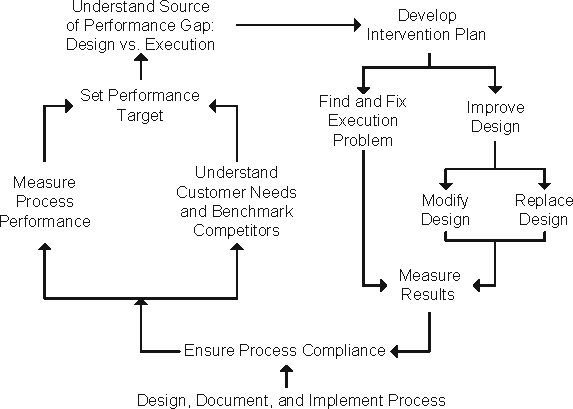
\includegraphics[width=0.8\textwidth]{Images/process_management_cycle.pdf}
\caption[Essentieller Zyklus der Geschäftsprozessmodellierung]{Essentieller Zyklus der Geschäftsprozessmodellierung \citep[S. 5]{Brocke2014}}
\label{process_management_cycle}
\end{figure}
\subsection{Business Process Mapping und Business Process Modeling}\label{subsec:BPMappingModeling}
Die Ermittlung und Visualisierung von Geschäftsprozessen stellt eine Teildisziplin im Management von Geschäftsprozessen dar. Gleichzeitig ist sie der Schlüssel zur Anpassung der Geschäftsprozesse, da ein genaues Verständnis der Abläufe für die Anpassung und Verbesserung unerlässlich sind \cite[vgl.][S. 6]{Jacka2009}. Mit dieser Problemstellung befassen sich sowohl Business Process Mapping als auch Business Process Modeling. Der Unterschied zwischen beiden besteht im wesentlichen in der Zielstellung und der damit verbundenen Abstraktionsebene \cite[vgl.][]{Smartdraw}. Process Mapping zielt im Kern auf die Dokumentation eines bestehenden Prozesses ab, weswegen das Unternehmen auf makroskopischer Sicht analysiert wird. Dabei werden die wesentlichen Funktionen und Rollen bei der Transformation des Inputs zum Output betrachtet. Process Modeling hingegen versucht bestehende Prozesse im Detail zu analysieren, um Engpässe aufzudecken und die Effizienz durch Anpassungen zu steigern \cite[vgl.][]{Appian}. Aus diesem Grund sind die dabei entstehenden Modelle detaillierter. Beide Disziplinen verwenden dabei im Idealfall standardisierte Beschreibungssprachen, wobei sich aus der höheren Detailtiefe beim Process Modeling eine höhere notwendige Komplexität der Beschreibungssprache ergibt. Aufgrund der vielen inhaltlichen und methodischen Überschneidungen der beiden Disziplinen kommt es leider häufig zu Verwechslungen beziehungsweise zur synonymen Verwendung beider Bezeichnungen \cite[vgl.][]{Smartdraw}.

Zu den allgemeinen Vorteilen von Process Mapping zählen die bessere Dokumentation der Prozesse, die Möglichkeit den Prozess grafisch zu visualisieren sowie die komplette Sicht auf die vielen verschiedenen Aspekte eines Prozesses \cite[vgl.][S. 8]{Jacka2009}. Neben diesen offensichtlichen Vorteilen gibt es allerdings noch zahlreiche weitere positive Aspekte, deren Wirkungsweise sich erst auf den zweiten Blick erschließt. Beispielsweise erhöht sich die Transparenz der Unternehmensprozesse, wodurch jeder Prozessteilnehmer seine Rolle im kompletten Kontext besser einschätzen kann. Dadurch wird die Wirkung der eigenen Tätigkeiten wesentlich klarer, was das Stolzgefühl der Mitarbeiter stärkt und so zu einer allgemeinen Steigerung der Mitarbeiterzufriedenheit führt. Zudem kann jeder Teilnehmer wesentlich mehr zur stetigen Verbesserung der Prozesse beitragen, da jedem ein holisitischer Blick auf den Prozess gewährt wird. Ein weiterer positiver Nebeneffekt ist die sich zwangsläufig ergebende Kundenorientierung, da für ein sinnvolles analysieren der Prozesse der Blick auf den für den Kunden generierten Output notwendig ist \cite[vgl.][S. 8-11]{Jacka2009}.

Prinzipiell besitzt auch Process Modeling ähnliche Vorteile, wie die bereits für Process Mapping aufgeführten. Aus der Abstraktionsebene und dem sich daraus ergebenden Detaillierungsgrad ergeben sich jedoch weitere Vorteile. Hierbei ist beispielsweise zu erwähnen, dass die Einarbeitung neuer Mitarbeiter durch die entsprechende Prozessdokumentation leichter fällt und dadurch Zeit eingespart werden kann. Durch die Modellierung der Prozesse entsteht sozusagen ein "`Prozesskatalog"' der auch als zentrales Nachschlagewerk fungieren kann. Zudem erlaubt der Detaillierungsgrad der Prozessmodelle, dass Teilaufgaben automatisiert werden können, was einen großen Vorteil darstellt. Dazu wird eine sogenannten Process Engine verwendet, die für den Nutzer beziehungsweise den Mitarbeiter als Schnittstelle zu genormten Prozessen fungiert. Standardaufgaben, wie beispielsweise das Weiterleiten eines Beurteilungsbogens nach der Prüfung, können dann automatisch durch die \ac{IT} ausgeführt werden \citep[vgl.][S. 2-8]{Freund2014}.

\subsection{BPMN 2.0}\label{subsec:BPMN}
Wie in den vorigen Abschnitten erwähnt wurde, nimmt die Visualisierung von Geschäftsprozessen einen wichtigen Standpunkt ein. \ac{BPMN} wird neben anderen Modellierungssprachen wie YAWL, EPK, Petrinetze, UML speziell im Rahmen des Business Process Modeling verwendet \cite[vgl.][S. 9]{Kossak2014}. Mit der ersten veröffentlichen Version im Jahre 2004 durch die \ac{BPMI} gilt BPMN als einer der jüngeren Vertreter der Prozessmodellierungssprachen. 2005 wurde die \ac{BPMI} durch die \ac{OMG} übernommen, die sich in der IT-Welt bereits durch die Entwicklung und Wartung von UML einen Namen gemacht hat. In der Folge wurde der Standard weiterentwickelt, bis er 2011 in der aktuellsten Version 2.0 verabschiedet werden konnte \citep[vgl.][S. 8f.]{Freund2014}. Die Aufnahme in den ISO 19510:2013 Standard und nicht zuletzt die Pflege der Sprache durch die OMG haben den Stellenwert der BPMN in der Vergangenheit stärken können und ihren Einfluss vergrößert \cite[vgl.][S.10f.]{Kossak2014}. Zudem scheint speziell im Vergleich mit anderen Modellierungssprachen der Fokus und der Blickwinkel der Sprache bei der Modellierung industrieller Prozesse am besten den Forderungen der Unternehmen zu entsprechen \cite[vgl.][S.16]{Kossak2014}. Der Vorteil liegt hier darin, dass BPMN eine angenehme Lösung für den Zielkonflikt zwischen Verständlichkeit für alle Betrachter und notwendiger Komplexität zur Modellierung detaillierter Zusammenhänge darstellt \citep[vgl.][S. 11f.]{Freund2014}.

Obwohl auch BPMN nicht fehlerfrei ist und der Standard teilweise Definitionslücken und Inkonsistenzen aufweist sowie fehlende Standardisierung bei den erstellten Modellen zu Inkompatibilitäten zwischen den verschiedenen Tools führt, erscheint es durchaus wahrscheinlich, dass sich diese Modellierungssprache in naher Zukunft als de facto Standard etablieren wird \cite[vgl.][S.161]{Kossak2014}.

Zur Unterstützung beim Verständnis der folgenden Kapitel folgt ein kurzer Überblick zu den Modellierungselementen und Konzepten von \ac{BPMN} 2.0. Der Standard, der auch die Grundlage für die folgenden Ausführungen bildet, wird von der \ac{OMG} in \citep{OMG2011} definiert.

\subsubsection{Elemente der Modellierung}\label{subsubsec:BPMNElemente}

Mit dem Fokus auf Einfachheit und Nachvollziehbarkeit werden die Elemente in \ac{BPMN} in die folgenden fünf Gruppen unterteilt:
\begin{enumerate}
\item Flussobjekte
\item Verbindende Objekte
\item Artefakte
\item Teilnehmer (Pools und Lanes)
\item Daten
\end{enumerate}
Ihre grafische Darstellung ist in Abbildung \ref{bpmn_basic_elements} zu sehen. Über eine Art visueller Notation in Gruppen ist es möglich, die Klasse oder Funktionalität von Elementen aufgrund ihrer Form einzuschätzen. Beispielsweise werden Ereignisse immer in Form eines Kreises dargestellt, wobei auch die Größendimension der verschiedenen Objekte gleich ist.
\begin{figure}[ht]
\centering
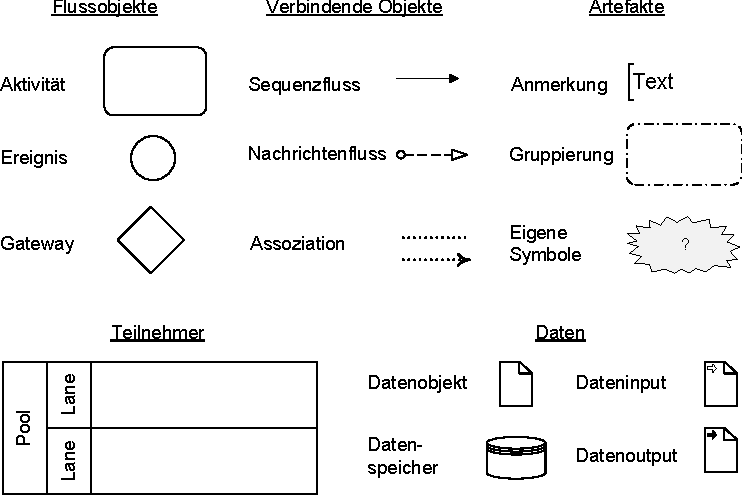
\includegraphics[width=1\textwidth]{Images/bpmn_basic_elements}
\caption[Die Basiselemente der BPMN 2.0]{Die Basiselemente der BPMN 2.0 \citep[S. 23]{Freund2014}}
\label{bpmn_basic_elements}
\end{figure}

Flussobjekte stellen die Kernelemente der Visualisierung dar und beschreiben das Verhalten des Geschäftsprozesses. Dazu unterteilen sich Flussobjekte in Aktivitäten, Ereignisse und Gateways \citep[vgl.][S. 29]{Laliwala2014}. Aktivitäten und Ereignisse erklären sich über ihren Namen sehr gut von allein und stehen somit stellvertretend für durchgeführte Aktionen (Aktivitäten) oder eintretende Ereignisse oder "`Dinge", 'die passieren können. Gateways wiederum stellen bedingte Verzweigungen dar und sind somit essentiell für komplexere Abläufe \citep[vgl.][S. 23]{Freund2014}.

Über den Sequenzfluss wird festgelegt, welche Elemente miteinander verbunden werden und in welcher Reihenfolge (angezeigt durch die Pfeilrichtung) die Elemente abgearbeitet werden. Diese Form des Prozessflusses findet allerdings nur innerhalb eines Pools oder einer Lane statt, weswegen für poolübergreifende Interaktionen Nachrichtenflüsse notwendig sind. Generell werden mit Pools und Lanes verschiedene Rollen, Personen oder andere Entitäten unterschieden und einzelne Elemente durch ihre Position innerhalb einer Lane oder eines Pools den entsprechenden Entitäten zugewiesen. Artefakte sollen zusätzliche Hinweise zum Prozess geben, ohne seine konkrete Ausführung zu verändern. Zur Verbindung von Artefakten mit anderen Objekten werden Assoziationen verwendet. Datenobjekte lassen darauf schließen, welche Daten im Laufe eines Prozesses entstehen oder verwendet werden und lassen sich ebenfalls über Assoziation mit Aktivitäten verknüpfen \citep[vgl.][S. 23f.]{Freund2014}. 
\subsubsection{Diagramm, Prozessmodell und -instanz}\label{subsubsec:BPMNModellInstanz}
Für das eindeutige Verständnis sollten die beiden Begriffe Prozessmodell und Prozessinstanz und der Unterschied zwischen beidem bekannt sein. Ein Prozessmodell beschreibt die modellierte Abbildung der Realität, also eines Prozesses, wovon ein oder mehrere in einem Diagramm enthalten sein können. Von einer Prozessinstanz wird gesprochen, wenn es um eine konkrete Ausführung eines Modells geht. Somit können mehrere Prozessinstanzen vom gleichen Prozessmodell aktiv sein. Man könnte dies auch als einen "`Vorgang"' beschreiben \citep[vgl.][S. 25f.]{Freund2014}.
\subsubsection{Token}\label{subsubsec:BPMNToken}
Das Token ist ein theoretisches Konzept, was bei der Analyse und dem Verständnis eines Prozessmodells hilft. Dabei stellt das Token ein Objekt dar, das in einem Start Event erstellt wird,  das Modell entlang der Fluss- und Verbindungselemente durchläuft und in der Regel durch ein End Event konsumiert wird. Solange ein Token im Prozessmodell "`unterwegs"' ist, bleibt die Instanz aktiv \citep[vgl.][S. 27]{OMG2011}. Gateways besitzen in diesem Zusammenhang eine besondere Bedeutung, da sie abhängig von ihrer Funktion Token vervielfachen oder verringern (konsumieren) können. Wie das Konzept des Tokens bei der Analyse verwendet wird, kann im folgenden Abschnitt bei der Erklärung eines konkreten Beispiels entnommen werden.
\subsubsection{Beispiel}\label{subsubsec:BPMNBeispiel}
Mit Hilfe eines Beispiels soll die Notation der BPMN und das Token-Konzept näher erläutert werden. Aus diesem Grund wurde ein Beispiel aus \citep{OMG2010} gewählt, welches allgemein leicht verständlich ist, aber trotzdem einen guten Querschnitt über die verfügbaren Modellierungselemente der BPMN 2.0 darstellt. Im gewählten Beispiel, das in Abbildung \ref{bpmn_pizza_collaboration} dargestellt wird, wird der Bestell- und Liefervorgang einer Pizza modelliert.
\begin{figure}[ht]
\centering
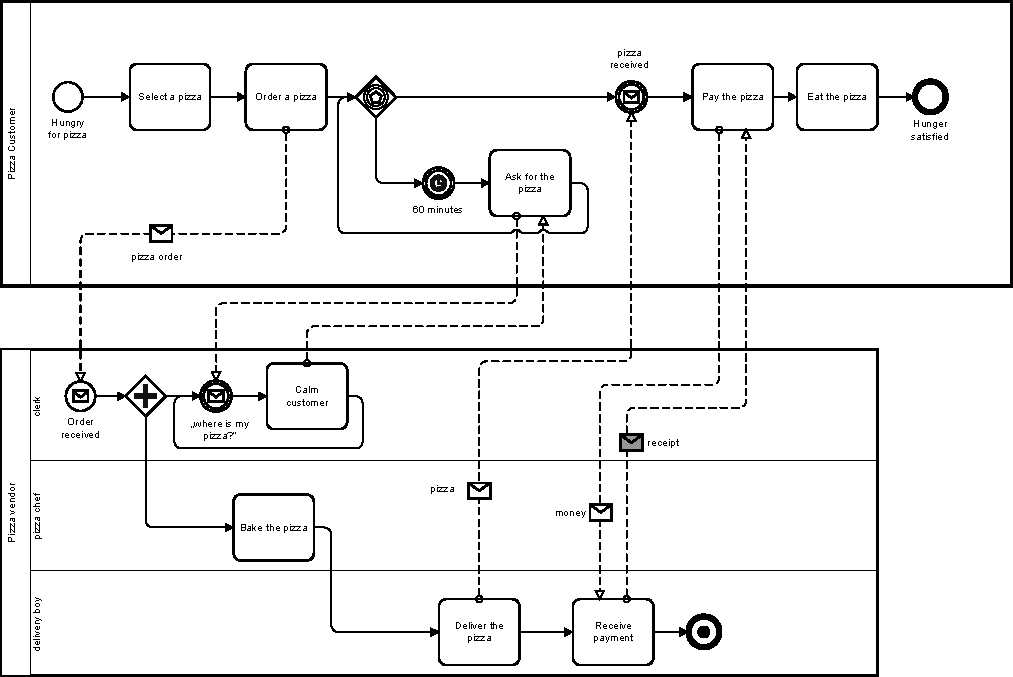
\includegraphics[width=1\textwidth]{Images/pizza_collaboration}
\caption[Bestell- und Liefervorgang einer Pizza]{Bestell- und Liefervorgang einer Pizza \citep[S. 4]{OMG2010}}
\label{bpmn_pizza_collaboration}
\end{figure}

Als erstes ist zu erkennen, dass der gesamte Prozess durch 2 Pools umgesetzt wird. Ein Pool symbolisiert in der BPMN immer eine übergeordnete Instanz, die die darin eingebetteten Lanes steuert. Eine Lane wiederum steht für eine Rolle im Prozess, die entsprechend ihrer Rolle Aufgaben durchführt oder abarbeitet. Diese Denkweise wird von dem Ziel der Automatisierung der Prozesse getrieben, da eine zentrale steuernde Instanz im Kontext eines Prozesses durch eine Process Engine sehr leicht abgelöst werden kann \citep[vgl.][S. 96ff.]{Freund2014}.

Das Startereignis liegt beim Konsumenten der Pizza, der Hunger auf eine Pizza verspürt. An dieser Stelle wird das Token generiert, was dann zu den nächsten Prozessschritten weiterläuft. Nachdem eine passende Pizza ausgewählt wurde, wird der eigentliche Bestellvorgang ausgelöst. Dazu wird, vermutlich durch einen Anruf oder per Onlinebestellung, eine Nachricht ("`pizza order"') für die Bestellung an den Angestellten des Pizzaverkäufers abgesetzt, was durch den gestrichelten Signalfluss und den Brief angezeigt wird. Anschließend wartet der Kunde auf seine Bestellung. Durch das eventbasierte Gateway wird abhängig vom ersten eingetroffenen Ereignis entweder der Bezahlvorgang eingeleitet (bei Erhalt der Pizza) oder beim Lieferanten nachgefragt, wo die Bestellung bleibt. Das Token verweilt somit im Gateway, bis eines der beiden Ereignisse ausgelöst wird, um dann dem ersten Ereignis zu folgen (XOR-Logik). Für den Bezahlvorgang wird ebenfalls der Austausch von Nachrichten zur Übergabe des Geldes und zum Erhalt der Zahlungsbestätigung verwendet. Anschließend kann der Kunde die Pizza essen und das Token wird im Abschlussevent konsumiert.

Auf der Seite des Pizzaverkäufers signalisiert der Erhalt der Nachricht für die Bestellung den Start. An dieser Stelle wird folglich das Token generiert und läuft in das parallele Gateway. Im parallelen Gateway wird das Token vervielfältigt und es startet auf jeder aus dem Gateway laufenden Prozesslinie ein Token. Eines der Token ist für die Beantwortung der Nachfragen des Kunden zuständig und wartet auf die entsprechende Nachricht, um den Kunden anschließend zu beruhigen. Das zweite Token läuft zum Pizzachef, der die bestellt Pizza bäckt. Danach wird der Prozess beim Botenjungen fortgesetzt, der die Pizza ausliefert und die Bezahlung erhält. Am Ende des Prozesses des Pizzaverkäufers gibt es mit dem Terminierungsereignis noch eine Besonderheit. In diesem Fall reicht ein normales Abschlussereignis nicht aus, da der Prozess ansonsten nie enden würde. Der Grund liegt in dem Zweig, der sich um die Kundennachfragen kümmert. Das Token, das aus dem parallelen Gateway in diese Schleife gestartet ist, kann niemals konsumiert werden, da es selbst nach Auslieferung der Pizza noch auf Nachfragen des Kunden warten würde. Aus diesem Grund wird mit Hilfe des Terminierungsereignisses der gesamte Prozess beendet und alle noch aktiven Token sofort gelöscht.

\section{Regulatorische Anforderungen für Medizingeräte}\label{sec:RegRequ}
Der Markt für Medizinprodukte gehört zu den stark reglementierten Märkten, in dem Unternehmen speziellen Anforderungen unterliegen. Prinzipiell ist dieses Thema sehr vielschichtig, da die Normen ein recht komplexes Gebilde erstellen, weswegen an dieser Stelle nur eine kurze Zusammenfassung mit eher oberflächlichen Betrachtungen, die für das Verständnis der folgenden Kapitel aber essentielle sind, gegeben werden kann.

Besonders wichtig und interessant ist hierbei die Frage wo die Grenzen dieses Marktes sind und welche Unternehmen und Produkte tatsächlich betroffen sind. Dazu finden sich in der Regel in den Normen und Standards entsprechende Definitionen, die eine Abgrenzung ermöglichen. Folgend ist ein Beispiel der \ac{GHTF} gegeben, welches den Begriff "`medizinisches Gerät (Medical Device)"' erläutert \citep[][S. 6]{GHTF2012}.
\begin{quote}
"`Medical device"' means any instrument, apparatus, implement, machine, appliance, implant, reagent for in vitro use, software, material or other similar or related article, intended by the manufacturer to be used, alone or in combination, for human beings, for one or more of the specific medical purpose(s) of:
\begin{itemize}
\item diagnosis, prevention, monitoring, treatment or alleviation of disease,
\item diagnosis, monitoring, treatment, alleviation of or compensation for an injury,
\item investigation, replacement, modification, or support of the anatomy or of a physiological process,
\item supporting or sustaining life,
\item control of conception,
\item disinfection of medical devices,
\item providing information by means of in vitro examination of specimens derived from the human body;
\end{itemize}
and does not achieve its primary intended action by pharmacological, immunological or metabolic means, in or on the human body, but which may be assisted in its intended function by such means.
\end{quote}

Aus dieser Definition leitet sich für medizinische Geräte eine besondere Verbindung zur Gesundheit des Patienten ab, was einen wesentlichen Unterschied zu anderen Märkten darstellt. Während beispielsweise auf dem Markt für Consumer Electronics die Funktionalität im Fokus des Anwenders und Kunden steht, ist es auf dem Markt für Medizintechnik die Sicherheit des Patienten, die genauso wichtig ist, wie der Kundennutzen beziehungsweise zusammen mit dem Risiko in einem angemessenen Verhältnis stehen muss. Oberstes Anliegen für eine Unternehmung ist jedoch bekanntermaßen in der Regel die Gewinnmaximierung, weswegen hier der Gesetzgeber eine wichtige Rolle übernimmt und die notwendige Sicherheit der Produkte einfordert. Das Ergebnis davon sind Standards und Normen, die vor der Markteinführung eines neuen Produktes erfüllt werden müssen \citep[vgl.][S. 3]{Higson2002}. Als Standard wird eine vereinbarte, wiederholbare Vorgehensweise bezeichnet, die durch ein Dokument festgelegt wird, das durch die Arbeit und Abstimmung eines verantwortlichen Ausschusses erarbeitet wird. Enthalten ist in der Regel eine technische Spezifikation oder andere präzise Kriterien, die als Regel, Richtlinie oder Definition fungieren.\citep[vgl.][S. 125-143]{Wong2013}.

Der Einsatz von Normen und Standards in der Medizintechnik ist kein neues Vorgehen, sondern hat sich über die letzten Jahrzehnte etablieren können. Die erste Anforderung zum Einsatz eines Qualitätsmanagementsystems wurde bereits 1976 in den USA eingeführt \citep[vgl.][S. 5]{Higson2002}.
\subsection{Sicherheit medizinischer Geräte}\label{subsec:Safety}
Wie bereits in Kapitel \ref{sec:RegRequ} angesprochen, besitzt die Sicherheit medizinischer Geräte eine besondere Bedeutung. Auch hierfür liefert die \ac{GHTF} eine Definition für eine essentielle Perspektive auf das Thema Sicherheit \citep[][S. 6]{GHTF2012b}.
\begin{quote}
Medical devices should be designed and manufactured in such a way that, when used under the conditions and for the purposes intended and, where applicable, by virtue of the technical knowledge, experience, education or training, and the medical and physical conditions of intended users, they will perform as intended by the manufacturer and not compromise the clinical condition or the safety of patients, or the safety and health of users or, where applicable, other persons, provided that any risks which may be associated with their use constitute acceptable risks when weighed against the benefits to the patient and are compatible with a high level of protection of health and safety.
\end{quote}
Aus dieser Definition geht klar hervor, dass die oberste Pflicht des Herstellers die Sicherstellung der Sicherheit für die Anwender und Patienten ist. Relativiert wird diese Aussage lediglich durch den Zusatz, dass Risiken immer im Verhältnis zum erwarteten Patientennutzen stehen müssen. Ein hohes Risiko für den Patienten ist somit nur akzeptabel, wenn die durchgeführten Aktionen zu einer bedeutenden Verbesserung des Gesundheitszustandes des Patienten führt. Diese Abwägung findet in einem entsprechenden Evaluierungsprozess vor der Markteinführung statt \citep[vgl.][S. 11]{Ramakrishna2015}. 

Absolute Sicherheit kann nicht garantiert werden, da jedes Gerät bis zu einem gewissen Grad ein Risiko in sich trägt und Fehler unter speziellen Umständen auftreten können. Aufgrund unvorhersehbarer Bedingungskonstellationen können Fehler unerwartet und zufällig auftreten, was selbst durch ausgiebige Tests im Vorfeld nicht ausgeschlossen werden kann. Deswegen wird versucht durch Risikobetrachtungen und -analysen die Gerätesicherheit sicherzustellen, indem die vom Gerät ausgehende Bedrohung durch Risikobewertungen abgeschätzt wird. Diese Form der Betrachtung wird auch unter Risikomanagement subsumiert, das sich in der Regel auf die Erfahrung von Experten für Medizintechnik stützt \citep[vgl.][S. 3]{Cheng2003}.

Aber nicht nur der Hersteller medizinischer Geräte allein trägt die Verantwortung für die Sicherheit. Jeder der betroffenen Stakeholder, bestehend aus Hersteller, Regierung, Öffentlichkeit/Patient, Benutzer und Verkäufer, trägt einen Teil zur Gewährleistung der Sicherheit bei. Diese Verantwortung ist in Abbildung \ref{qs_shared_resp} veranschaulicht. Die Rolle des Herstellers ist vermutlich die größte und liegt durch das Design, die Entwicklung und die Produktion des Produktes klar auf der Hand. Die Regierung ist dafür zuständig, dass die in dem jeweiligen Land verfügbaren Geräte sicher und nützlich sind. Der Verkäufer hat als Schnittstelle zwischen Hersteller und Benutzer eine besondere Verantwortung, durch die Überwachung der Konformität zu den regulatorischen Normen und der Bereitstellung des Kundenservice. Der Nutzer des Gerätes wiederum muss sicherstellen, dass er die Funktion des Gerätes erfasst hat und es sicher bedienen kann. Auf den ersten Blick mag es nicht sofort ersichtlich sein, in welcher Weise die Öffentlichkeit und der Patient die Sicherheit beeinflussen können, aber auch der gesellschaftliche Druck auf einen Hersteller zur Erfüllung einer entsprechenden Norm kann am Ende zur Erhöhung der Produktsicherheit beitragen \citep[vgl.][S. 7f.]{Cheng2003}.
\begin{figure}[ht]
\centering
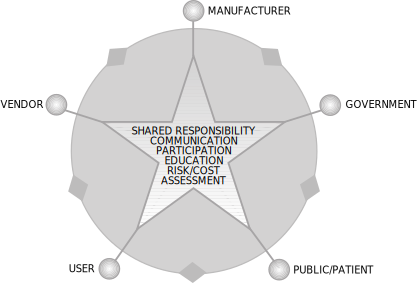
\includegraphics[width=1\textwidth]{Images/qs_shared_resp}
\caption[Ideale Bedingungen zur Sicherstellung der Sicherheit medizinischer Geräte]{Ideale Bedingungen zur Sicherstellung der Sicherheit medizinischer Geräte \citep[S. 8]{Cheng2003}}
\label{qs_shared_resp}
\end{figure}
\subsection{Gründe und Bedeutung der Regulierung für Medizinprodukte}\label{subsec:Gruende}
Der Hauptgrund für regulative Normen in der Medizintechnik wurde mit der Verantwortung gegenüber der Patientensicherheit bereits genannt. Dieses Ziel stellt hohe Forderungen an die Hersteller, um die Sicherheit zu gewährleisten. Zur Erfüllung der Anforderungen müssen die Hersteller hohe Aufwände in Kauf nehmen. Interessanterweise hat Regulierung und vor allem Harmonisierung der Normen für die Hersteller aber auch große Vorteile. Durch die Harmonisierung der Normen ist es für die Unternehmen wesentlich einfacher den Marktzugang für ihre Produkte in vielen verschiedenen Ländern zu erreichen. Vor allem im Zeitalter der Globalisierung ist dieser Aspekt sehr wichtig geworden. Würde jeder Gesetzgeber komplett eigene Richtlinien erlassen wäre der Aufwand für die Hersteller immens, wenn sie pro Land und Produkt einen eigenen kompletten Zulassungsprozess durchlaufen müssten.

Aus diesen Gründen werden Standards eingesetzt, die unter anderem Referenzkriterien schaffen. Erst durch die Festlegung von festen Kennzahlen beziehungsweise messbaren Anforderungen kann die Leistung und Erfüllung von Kriterien transparent werden. Dies ermöglicht danach den Vergleich von Produkten und das Schaffen von Fakten durch die Erfüllung der gestellten Anforderungen. Zudem werden dadurch Informationen bereitgestellt, die die Sicherheit, Verlässlichkeit und Leistung des Produktes oder Services erhöhen. Dies fördert auch für den Nutzer und/oder Patienten die Transparenz über die Gerätecharakteristika. Es kann somit viel besser eingeschätzt werden, welche Eigenschaften ein Produkt hat und, dass für die Bedienung wichtige Anforderungen erfüllt sind, was das Vertrauen bei der Benutzung erhöht. Nebenbei erhält der Konsument die Möglichkeit Produkte eines Herstellers durch die Produkte eines anderen auszutauschen \citep[vgl.][S. 19.]{Cheng2003}.

Zur Prüfung der Konformität mit einem Standard gibt es vier verschiedene Möglichkeiten, die sich jeweils auf verschiedene Abstraktionsebenen beziehen. Die Konformität eines Produktes kann durch direkte Tests sichergestellt werden. Prozesse wiederum können mit Audits geprüft werden, die entweder durch gesonderte Organisationen oder regulatorische Autoritäten durchgeführt werden, die ein entsprechendes Siegel bei Erfüllung vergeben. Ganze Managementsysteme werden auch über Audits geprüft und führen bei Erfüllung der Anforderungen zu Registrierungen in zentralen Karteien (z.B. ISO13485/ISO9001). Die letzte Möglichkeit ist in der Akkreditierung zu sehen, die einer Organisation oder einer Person die formale Erlaubnis erteilen, eine spezielle Aufgabe auszuführen. Ein Beispiel hierfür sind die benannten Stellen in der europäischen Union, die im Medizintechniksektor die Produktkonformitätsprüfung durchführen können, nachdem sie durch eine Autorität des Staates dazu ermächtigt wurden \citep[vgl.][S. 19f]{Cheng2003}.

Prinzipiell kann zwischen verpflichtenden und freiwilligen Standards unterschieden werden. Ein Standard kann durch ein Unternehmen, eine Gesellschaft, Verbände oder ähnliche Institutionen festgelegt werden. Ein Standard kann durch den Gesetzgeber aufgegriffen werden und als verpflichtend eingestuft werden, womit er im jeweiligen Gesetz verankert wird. Die meisten der Standards sind momentan freiwillig, da die Festlegung von Standards als verpflichtende Normen weitreichende Konsequenzen für den globalen Handel hat. Außerdem bedienen die verpflichtenden Vorschriften der Behörden zwar die wesentlichen Sicherheits- und Leistungsprinzipien, dies reicht den Hersteller aber in der Regel nicht aus, da diese noch detailliertere Spezifikationen benötigen. Diesen Detaillierungsgrad können die Behörden aber aufgrund fehlender Ressourcen und Expertise nicht liefern, weswegen freiwillige Standards von den betroffenen Parteien entwickelt werden. Die Vorteile freiwilliger Standards sind vielfältig und liegen beispielsweise darin, dass der Standard von Experten entwickelt wird, die direkten Zugang zu den betroffenen Entitäten besitzen. Zudem wird der weltweite Zugriff auf neue Technologien verbessert, da der Prozess der Harmonisierung der regulatorischen Anforderungen vereinfacht wird. Ein weiterer Vorteil ist darin zu sehen, dass es viel einfacher ist, einen Standard zu aktualisieren, als die Gesetzgebung anzupassen. Die Anpassung des Standards obliegt dem Zusammenschluss von Experten, der ihn entwickelt hat \citep[vgl.][S. 19-22]{Cheng2003}.

Ein Beispiel für eine Organisation, die sich mit der Festlegung von freiwilligen Standards beschäftigt ist das \ac{IMDRF}, das 2012 die \ac{GHTF} abgelöst hat. Das \ac{IMDRF} beschäftigt sich beispielsweise damit fundamentale Definitionen und Frameworks zu erarbeiten \citep[vgl.][]{Hall2014}.
\subsection{Überblick über die wichtigsten Standards}\label{subsec:UeberblickStandard}
In Zeiten der Globalisierung wäre es für die Hersteller undenkbar, für jedes Land eine separate Prüfung der Konformität nach nationalem Recht durchzuführen, weswegen von der Industrie Standardisierung gefordert wird \citep[vgl.][S. 6]{Higson2002}. Weltweit gibt es viele verschiedene Organisationen, die sich mit der Normierung beschäftigen und Standards verabschieden. Allerdings ist vorher meist nicht klar, welcher Standard sich durchsetzt und sich im Markt etablieren kann. Zu den wichtigsten Vertretern zählen die ausgearbeiteten Standards der \ac{ISO}. Abbildung \ref{iso_standards} liefert einen Überblick über die wichtigsten Normen für medizinische Geräte.
\begin{figure}[ht]
\centering
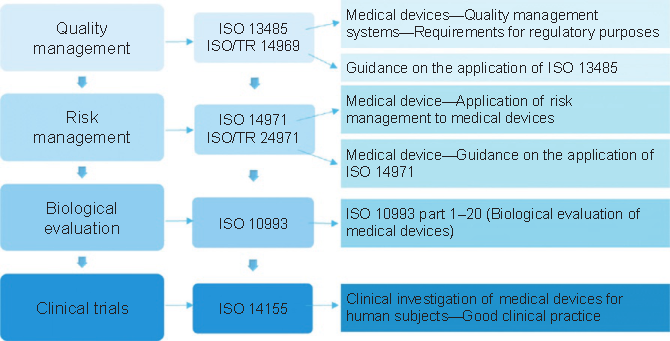
\includegraphics[width=1\textwidth]{Images/iso_standards}
\caption[ISO Standards für medizinische Geräte]{ISO Standards für medizinische Geräte \citep[S. 16]{Ramakrishna2015}}
\label{iso_standards}
\end{figure}
Diese Standards bilden häufig die Grundlage für die Erstellung nationaler Normen. Dabei kann der entsprechende Standard entweder als verpflichtend festgelegt werden oder er wird in eigene Vorschriften des Gesetzgebers überführt, was in Abbildung \ref{iso_standards_adaption} gut erkannt werden kann.
\begin{figure}[ht]
\centering
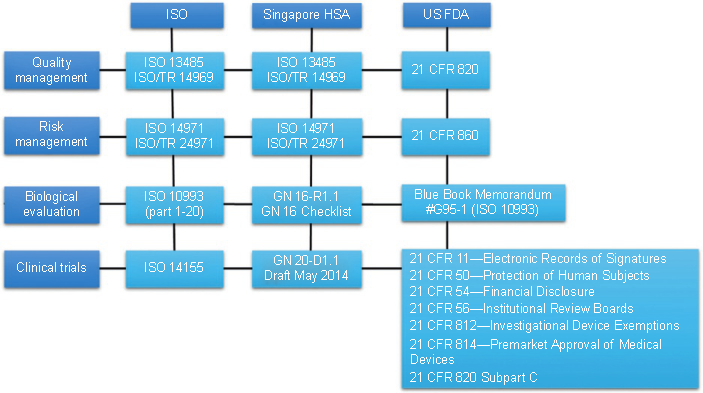
\includegraphics[width=1\textwidth]{Images/iso_standards_adaption}
\caption[Standards und Normen für medizinische Geräte]{Standards und Normen für medizinische Geräte \citep[S. 16]{Ramakrishna2015}}
\label{iso_standards_adaption}
\end{figure}

Zu den wichtigsten nationalen Vertretern mit umfassendem Regulierungssystem zählen \citep[vgl.][S. 14]{Ramakrishna2015}:
\begin{itemize}
\item USA (Food \& Drug Administration(FDA), Center for Devices \& Radiological Health (CDRH))
\item Kanada (Therapeutic Products Directorate)
\item EU (European Commission Directorate, Mitgliedsstaaten)
\item Japan (Ministry of Health, Labour \& Welfare (MHLW), Pharmaceuticals \& Medical Devices Agency (PMDA))
\item Australien (Therapeutic Goods Administration (TGA))
\item China (China Food \& Drug Administration (CFDA))
\item Indien (Drug Controller General of India (DCGI), Central Drugs Standard Control Organization (CDSCO))
\item Singapur (Health Science Authority (HSA))
\end{itemize}

Ein Vorgehen, das sich bei all diesen Vertretern bewährt hat, ist die Einteilung der medizinischen Geräte in verschiedene Risikoklassen, was über den Grad der Kontrollmechanismen und die damit verbundenen Anforderungen an die Hersteller entscheidet (siehe Abbildung \ref{classification_meddev}).
\begin{figure}[ht]
\centering
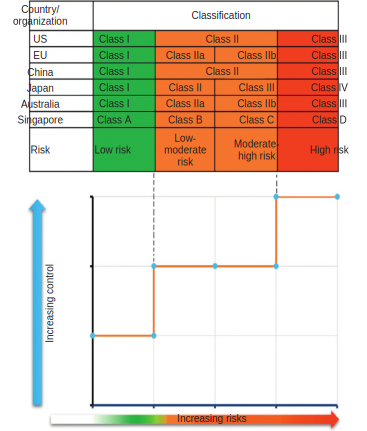
\includegraphics[width=0.7\textwidth]{Images/classification_meddev}
\caption[Einteilung medizinischer Geräte in verschiedene Risikoklassen]{Einteilung medizinischer Geräte in verschiedene Risikoklassen \citep[S. 22]{Ramakrishna2015}}
\label{classification_meddev}
\end{figure}

Diese Arbeit beschäftigt sich im Kern mit den Anforderungen der \ac{MDR} 2017/745, die von der Europäischen Kommission erstellt wurde. Der Fokus liegt somit auf den Regeln in Europa und nicht auf den Statuten der FDA, obwohl diese aktuell aufgrund der Tatsache, dass der Markt in den USA das größte finanzielle Volumen aufweist \citep[vgl.][S. 8]{ITA2016}, weltweit die vermutlich wichtigste Rolle einnimmt.

Die Situation auf dem europäischen Markt ist etwas komplexer als in den USA, da die FDA dort als Regierungsunternehmen direkte Befugnisse besitzt. In der EU gibt es neben dem Hersteller insgesamt drei verschiedene Rollen, die für die Regulierung relevant sind. Die Zusammenhänge zwischen europäischer Kommission, staatlicher Behörde, benannter Stelle und Hersteller sind in Abbildung \ref{regulativ_structure_eu} dargestellt. Daraus ist ersichtlich, dass die benannte Stelle für den Hersteller eine sehr wichtige Rolle einnimmt, da sie zum einen den Hersteller überwacht und zum anderen die erstellten Produkte prüft. Die benannten Stellen wiederum werden durch die staatlichen Behörden zugelassen und kontrolliert. Die Europäische Kommission als oberste Instanz legt die zu erfüllenden Normen fest, die von den staatlichen Behörden umgesetzt werden.
\begin{figure}[ht]
\centering
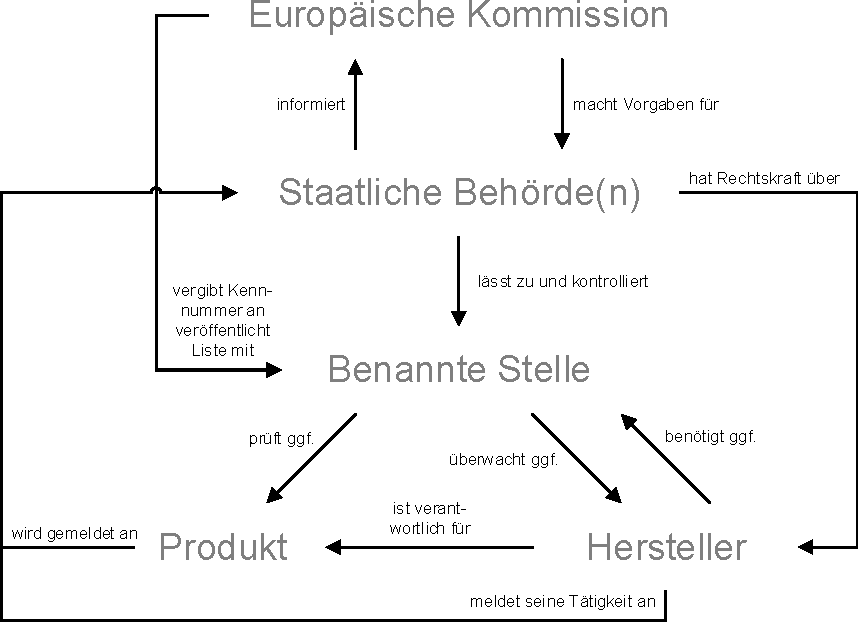
\includegraphics[width=0.7\textwidth]{Images/regulativ_structure_eu}
\caption[Beziehung zwischen Kommission, staatlicher Behörde, benannter Stelle und Hersteller auf dem Medizintechnikmarkt in Europa]{Beziehung zwischen Kommission, staatlicher Behörde, benannter Stelle und Hersteller auf dem Medizintechnikmarkt in Europa \citep[S. 38]{Johner2015}}
\label{regulativ_structure_eu}
\end{figure}

Auf dem Weg zu einem verkaufsfähigen Produkt müssen neben der eigentlichen Entwicklung und Produktion verschiedene Stufen in der europäischen Union durchlaufen werden. Der erste Schritt besteht in der Auswahl der passenden Direktive der europäischen Kommission. Anschließend muss die Risikoklasse bestimmt werden, die die Ausprägung der folgenden Schritte festlegt oder ob sogar Schritte übersprungen werden dürfen. Um die Konformitätsbescheinigung zu erhalten, muss eine Prüfung durch die benannte Stelle erfolgen, die zunächst durch den Hersteller ausgewählt werden muss. Eine Liste der möglichen benannten Stellen wird dazu von der europäischen Kommission zur Verfügung gestellt. Nach erfolgreicher Prüfung erhält der Hersteller die CE-Kennzeichnung, die ihm die Konformität zu den Anforderungen der europäischen Kommission und den erfolgreichen Abschluss der Prüfungen bescheinigt. Mit dieser Bescheinigung kann das Produkt auf dem Markt platziert werden. Während das Produkt im Markt ist, ist der Hersteller zur Meldung von unerwünschten Zwischenfällen und zur ständigen Beobachtung anhand von klinischen Studien verpflichtet \citep[vgl.][S. 32f]{Ramakrishna2015}.
\begin{figure}[ht]
\centering
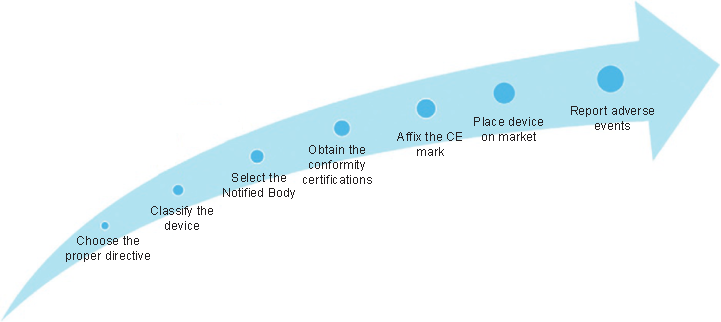
\includegraphics[width=1\textwidth]{Images/route_assure_compliance}
\caption[Route zur Erfüllung regulatorischer Anforderungen für medizinische Geräte in der EU]{Route zur Erfüllung regulatorischer Anforderungen für medizinische Geräte in der EU \citep[S. 33]{Ramakrishna2015}}
\label{route_assure_compliance}
\end{figure}

Der zentrale Rechtsrahmen zur Zulassung medizinischer Geräte in der EU bestand bisher aus den folgenden drei Direktiven, die über die Zeit mehrfach angepasst wurden \citep[vgl.][S. 32]{Ramakrishna2015}:
\begin{itemize}
\item Direktive 90/385/EWG (aktive implantierbare medizinische Geräte)
\item Direktive 93/42/EWG (medizinische Geräte)
\item Direktive 98/79/EG (in vitro diagnostische medizinische Geräte)
\end{itemize}
Durch die neue MDR 2017/745 werden die Direktiven 90/385/EWG und 93/42/EWG ersetzt. Auch die Direktive 98/79/EG wird ersetzt, bekommt mit der IVDR 2017/746 eine eigene Verordnung \citep[vgl.][]{Johner2018}.
\subsection{Auswirkungen auf die Entwicklung und den Produktlebenszyklus}\label{subsec:AuswirkungenAufEntwicklung}
Die vorangegangenen Kapitel haben klargestellt, dass sich Hersteller medizinischer Produkte in einem stark reglementierten Markt bewegen. Die Verantwortung dem Patienten gegenüber und die Anforderungen der Autoritäten schlagen sich in weitreichenden Konsequenzen für den Entwicklungs- und Produktionsprozess nieder. Das Maß der Beeinflussung kann beispielsweise am Fokus der verschiedenen Studiengruppen der GHTF erkannt werden. Auch wenn diese mittlerweile nicht mehr existiert, dient sie immernoch als Vorlage und Querschnitt über die Bemühungen solcher Organisationen. Aus Abbildung \ref{ghtf_focus} ist ersichtlich, dass die Arbeitsgruppen jeweils verschiedene Schwerpunkte setzen (dargestellt als durchgezogene Linie). Über die gestrichelten Linien wird angezeigt, dass der Einfluss jeder Gruppe prinzipiell in jedem Tätigkeitsbereich zu finden ist.
\begin{figure}[ht]
\centering
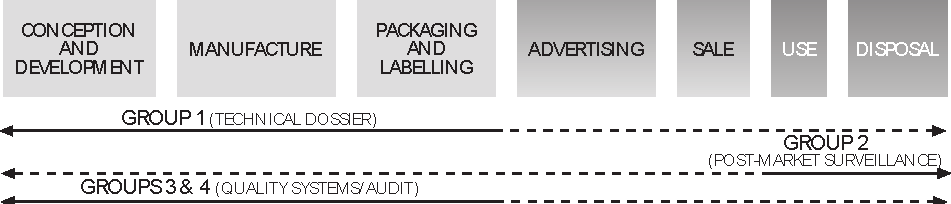
\includegraphics[width=1\textwidth]{Images/ghtf_focus}
\caption[Fokus der verschiedenen Studiengruppen der GHTF]{Fokus der verschiedenen Studiengruppen der GHTF \citep[S. 16]{Cheng2003}}
\label{ghtf_focus}
\end{figure}

Die Anforderungen an den Entwicklungsprozess eines Unternehmens verlangen einen durchgängigen Nachweis der Entwicklungssystematik. In den Normen werden dabei keine konkreten Vorschriften zur Umsetzung gegeben, sondern höchstens unverbindliche Hinweise zur möglichen Umsetzung. Dies stellt die Unternehmen zwar vor große Herausforderungen, lässt ihnen jedoch auch Freiräume bei der Umsetzung. In jeder Hinsicht muss berücksichtigt werden, dass das Ziel entsprechender Normen darin besteht, die Sicherheit der Geräte zu bewerkstelligen und nicht die Gewinnmaximierung der wirtschaftenden Unternehmen durch die Bereitstellung einfacher und günstiger Prozesse in der Entwicklung und Herstellung voranzutreiben. Abhängig von den eigenen individuellen Bedingungen (z.B. Unternehmensgröße, Kultur, spezielle Unternehmensrichtlinien) muss somit jedes Unternehmen nach einer eigenen kostengünstigen und effizienten Lösung suchen \citep[vgl.][S. 103-107]{Johner2015}.

Der Schwerpunkt dieser Arbeit liegt auf der Rückwirkung der nachgelagerten Qualitätsprozesse auf den Entwicklungsbereich, weswegen mit dem Requirements Engineering und dem Product Lifecycle Management folgend die Auswirkungen auf die dafür wichtigsten Schnittstelle im Unternehmen kurz beleuchtet werden sollen.
\subsubsection{Requirements Engineering und Änderungsmanagement}
Generell beschäftigt sich das Requirements Engineering mit dem Erheben und Pflegen der Anforderungen für die Entwicklung eines Produktes. Für das Hauptthema dieser Arbeit soll an dieser Stelle die Bedeutung der Traceability herausgehoben werden, die für die Nachverfolgbarkeit der Anforderungen steht. "`Unter Traceability versteht man die Nachvollziehbarkeit von Entscheidungen und Abhängigkeiten vom Projektbeginn bis Projektende über alle Informationen und Repräsentationsformen der Darstellung."'\citep[][S. 407]{Rupp2002} Zu jedem Zeitpunkt einer Entwicklung muss es somit möglich sein, die Quelle für eine entsprechende Anforderung zu ermitteln, was im Rahmen der durch die Autoritäten geforderten Entwicklungssystematik für den Hersteller verpflichtend ist \citep[vgl.][S. 117]{Johner2015}. Dabei wird zwischen horizontaler und vertikaler Traceability unterschieden. Vertikale Traceability betrachtet die Beziehungen zwischen Elementen (z.B. Anforderungen) auf verschiedenen Abstraktionsebenen, womit beispielsweise geklärt werden kann, welcher Test welche Anforderung abdeckt und woher die Anforderung stammt. Horizontale Traceability wiederum stellt die Nachverfolgbarkeit von Elementen vom gleichen Typ und auf gleicher Ebene her (z.B. die Bereitstellung der Versionshistorie für jedes einzelne Requirement) \citep[vgl.][]{Ebert2014}. Solange ein Produkt noch nicht verkauft wird, sind Informationen wie die Versionshistorie zu jedem Item relativ uninteressant. Dies ändert sich jedoch mit der erfolgten Zulassung, denn für Änderungen, die nach der Zulassung erfolgen, muss eine lückenlose Dokumentation erstellt werden. Meist sind solche Änderungen das Ergebnis der "`post-market"' Prozesse, die in Kapitel \ref{sec:PMProzesse} genauer erläutert werden. In der Dokumentation muss beispielsweise erläutert werden, aufgrund welchen Fehlers eine Änderung durchgeführt wurde. Zudem muss die Genehmigung der Änderung anhand der Aufzeichnungen des Entscheidungsgremiums nachvollziehbar sein \citep[vgl.][S. 145f.]{Johner2015}. Dieser ist Prozess allgemein unter dem Namen Änderungswesen (Engineering Change Management) oder Änderungskontrolle bekannt.

Das Änderungswesen ist eine koordinierte Verwaltungsdisziplin, die sich darauf versteht produktbezogene Änderungen zu überwachen. Ziel des Änderungsmanagements ist es demnach Ideen zu sammeln, daraus Lösungsansätze zu erstellen und diese auf ihre technischen und wirtschaftlichen Folgen hin zu untersuchen \citep[vgl.][S. VII]{Prostep2007}. Welch großen Einfluss das Änderungsmanagement für die Entwicklung und Produktion besitzt wird in Abbildung \ref{plm_process_map} deutlich.
\begin{figure}[ht]
\centering
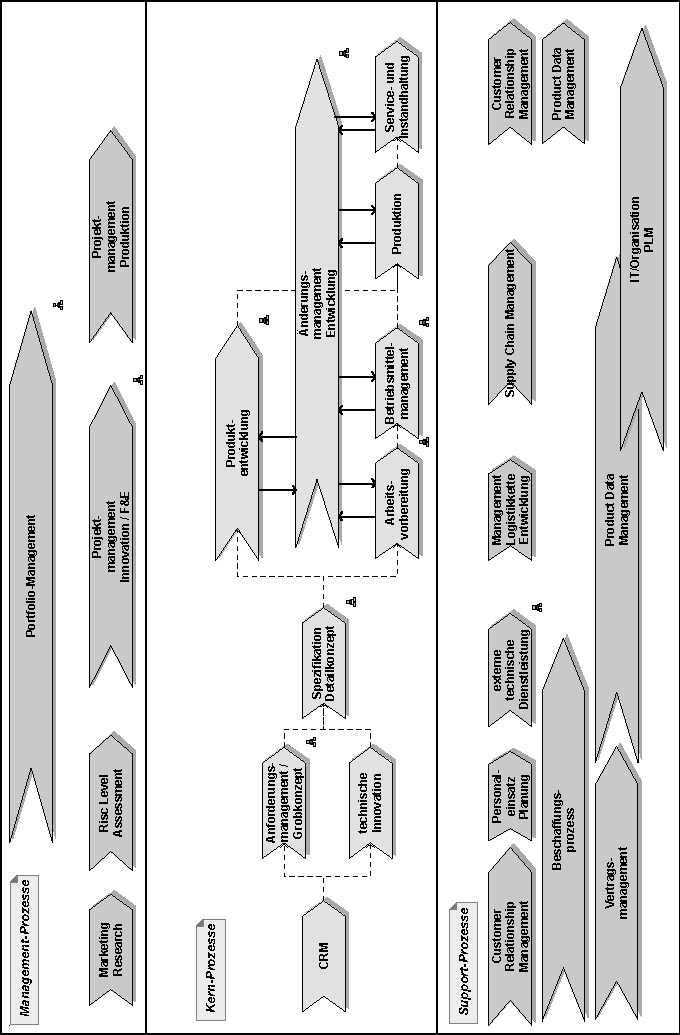
\includegraphics[height=0.9\textheight]{Images/plm_process_map}
\caption[Prozesslandkarte PLM]{Prozesslandkarte PLM \citep[S. 36]{Scheer2006}}
\label{plm_process_map}
\end{figure}
In der gesamten Prozesslandkarte besitzt das Änderungsmanagement neben der Produktentwicklung weitere Schnittstellen zur Arbeitsvorbereitung, dem Betriebsmittelmanagement, der Produktion und dem Service und der Instandhaltung. Über die Ausprägung des Änderungsprozesses gibt es keinen klaren Konsens, so dass sich verschiedene Formen entwickelt haben, die sich schon allein in der Anzahl der Prozessschritte deutlich unterscheiden. Mindestens besteht der Prozess demnach aus 3 Schritten, aber auch Beispiele mit bis zu 19 Schritten sind bekannt \citep[vgl.][S. 155]{Stark2015}.

Höchste Anforderungen stellt das Änderungsmanagement dabei an die IT, denn die Auswirkungen von veränderten Anforderungen müssen einfach ersichtlich sein und Transparenz sollte möglichst über eine direkte Navigation gegeben sein. Die oberste Anforderung besteht darin auch nach einer Produktänderung konsistente Daten sicherzustellen, um alle historischen Änderungszustände reproduzierbar zu machen \citep[vgl.][S. 85]{Scheer2006}.
\subsubsection{Product Lifecycle Management}
Das \ac{PLM} stellt den Geschäftsprozess dar, der die Produkte eines Hersteller über die erste Produktidee bis zur Abkündigung während ihres gesamten Lebenszyklus begleitet \citep[vgl.][S. 203]{Kale2016}. Zu den Kernfunktionen zählen zum Beispiel das Produktstrukturmanagement, das Dokumentenmanagement, das Änderungsmanagement oder das Workflowmanagement \citep[vgl.][S. 44]{Saaksvuori2008}. Das Änderungswesen stellt häufig einen der zentralsten Prozesse dar, wie auch in der Medizintechnik, da die Pflege von Änderungen eine grundlegende Anforderung für die Hersteller ist \citep[vgl.][S. 175]{Arnold2011}. Der Fokus von \ac{PLM} liegt somit auf Datenmanagement, denn der Kern der PLM Prozesse unterstützt die Aufnahme, Organisation und Wiederverwendung von Wissen über den gesamten Produktlebenszyklus \citep[vgl.][S. 46]{Tayaran2012}.

In Bezug auf Datenmanagement besitzen Informationsflüsse einen speziellen Stellenwert. Häufig sind Informationsflüsse im Anschluss an die Produktauslieferung zum Hersteller nahezu abgeschnitten, wodurch wichtige Informationen aus dem Service und der Wartung verloren gehen und nicht in die Entwicklung und Produktion eingepflegt werden \citep[vgl.][S. 16f.]{Jun2012}. Dieses Vorgehen ist in der Medizintechnik jedoch nicht akzeptabel, da durch die regulativen Anforderungen speziell dieser Informationsfluss in Verbindung mit dem Änderungswesen einen sehr hohen Stellenwert besitzt.
\section{Qualitätsprozesse nach Markteinführung medizinischer Geräte}\label{sec:PMProzesse}
- QMS soll generell Qualität sicherstellen; QMS beeinflusst alle Phasen die den Lebenszyklus eines Produktes betreffen --> dazu gehören auch Aktivitäten nach Markteinführung\citep[vgl.][S. 13]{Cheng2003}
- dabei prägen sich die Prozesse in korrigierende und präventive Maßnahmen aus \citep[vgl.][S. 338-350]{Abuhav2012}

- Besonderheit bei Medizinprodukten ist die Sorgfaltspflicht der Hersteller, dass kein Patient zu Schaden kommen soll
- Deswegen ist Entwicklung und auf den Markt bringen die eine Sache, aber danach gibt es für die Hersteller neben den üblichen Anforderungen an Support, die für Hersteller aller Branchen gelten kritische Pflichten, die die Sicherheit für die Patienten sicherstellen soll
- Hauptvorteil dafür QMS zu bemühen liegt im präventiven Charakter, der wesentliche Effizienvorteile gegenüber reaktiven Ansätzen der Kontrollen am Ende der Fertigungslinie aufweist\citep[vgl.][S. 14]{Cheng2003}

- ISO 13485:2016, ISO 14971:2012, von FDA gibt es separates Guidance Dokument, MDR stellt auch Forderungen \citep[vgl.][]{Johner2017}
- vor allem in Europa war zuletzt die Gesetzeslage in diesem Kontext nicht zufriedenstellend vor der Verabschiedung der MDR, da fehlende Transparenz und uneindeutige Festlegungen zu viel Spielraum gelassen haben \citep[vgl.][S. 1]{Chowdhury2014}

- Anforderungen bestehen dabei für allgemeines Vorgehen in festgehaltenen Plänen und genauen Vorgaben, wie mit Zwischenfällen umzugehen ist, da diese mitunter an zentralen Stellen angezeigt werden müssen

- Gehören zu Aufgaben des QMS

- Allgemeines Ziel ist es die Qualität der Produkte zu gewährleisten notwendige Daten zu sammeln, zu evaluieren und über folgende Aktionen zu unterscheiden --> dabei wird in der Regel zwischen korrigierenden und präventiven Aktionen unterschieden
\subsection{Post Market Surveillance}\label{subsec:PMS}
- Suche und Detektion von Problemen des medizinischen Gerätes, die nicht vor Markteinführung erkannt wurden \citep[vgl.][S. 213]{DeMarco2011}

- Anders als in vorheriger Medical Devices Directive wird in MDR eine Definition für PMS gegeben \citep[vgl.][S. 1]{Pugh2017}
\begin{quote}
Deutsche Übersetzung aus MDR 
Definition PMS:
"`Überwachung nach dem Inverkehrbringen"' bezeichnet alle Tätigkeiten, die Hersteller in Zusammenarbeit mit anderen Wirtschaftsakteuren durchführen, um ein Verfahren zur proaktiven Erhebung und Überprüfung von Erfahrungen, die mit den von ihnen in Verkehr gebrachten, auf dem Markt bereitgestellten oder in Betrieb genommenen Produkten gewonnen werden, einzurichten und auf dem neuesten Stand zu halten, mit dem ein etwaiger Bedarf an unverzüglich zu ergreifenden Korrektur- oder Präventivmaßnahmen festgestellt werden kann. \citep[Kapitel 1 Artikel 2 60.]{MDR2017}
\end{quote}

Sehr guter Absatz, aber muss noch angepasst werden, um nicht alles direkt zu kopieren \citep[vgl.][]{Johner2017}
Hersteller müssen die Risiken durch ihre Medizinprodukte minimieren und die Sicherheit der Patienten gewährleisten, bevor sie ihre Produkte in den Markt bringen. Behörden und benannte Stellen überprüfen dies im Rahmen der Zulassung bzw. Konformitätsbewertung.

- Benutzer vor Risiken beschützen, aber auch Vorteile für Hersteller, da Leistung der Produkte überwacht wird und dadurch die Qualität verbessert werden kann und Kosten reduziert werden können \citep[vgl.][S. 2]{Pugh2017}

Allerdings offenbaren sich einige Risiken erst später im Laufe der Zeit, wenn die Anwender die Produkte täglich einsetzen.

Die Post-Market Surveillance hat zum Ziel,
- diese Risiken beim praktischen Gebrauch des Produktes systematisch zu identifizieren,
- die Leistungsfähigkeit der Produkte „im Feld“ zu überprüfen,
- Produktfehler und unentdeckt gebliebene Sicherheitsprobleme zu finden,
- die Nutzen-Risiko-Bewertung kontinuierlich zu aktualisieren und
- notwendige Maßnahmen wie Rückrufe schnell einzuleiten.
\citep[vgl.][]{Johner2017}

Zu den Datenquellen gehören \citep[vgl.][S. 285-288]{Abuhav2012}
 - Distributoren
 - Kundenbefragungen
 - Service Telefonate
 - Produktbewertungen und Audits
 - Veröffentlichungen in Journalen, Literatur und Fachartikel
 - Forschung und klinische Bewertung
 - Kundenbeschwerden
 - Rückrufe medizinischer Geräte

\subsection{Post Market Clinical Follow-Ups}\label{subsec:PMCF}
Zitat aus MDR:
\begin{quote}
Die klinische Nachbeobachtung nach dem Inverkehrbringen ist als ein fortlaufender Prozess zur Aktualisierung der klinischen Bewertung gemäß Artikel 61 und Teil A dieses Anhangs zu verstehen und wird im Plan des Herstellers zur Überwachung nach dem Inverkehrbringen behandelt. Bei der klinischen Nachbeobachtung nach dem Inverkehrbringen sammelt und bewertet der Hersteller auf proaktive Weise klinische Daten, die aus der Verwendung eines die CE-Kennzeichnung tragenden, im Rahmen seiner Zweckbestimmung gemäß dem einschlägigen Konformitätsbewertungsverfahren in den Verkehr gebrachten oder in Betrieb genommenen Produkts im oder am menschlichen Körper hervorgehen, um die Sicherheit und die Leistung während der erwarteten Lebensdauer des Produkts zu bestätigen, die fortwährende Vertretbarkeit der ermittelten Risiken zu gewährleisten und auf der Grundlage sachdienlicher Belege neu entstehende Risiken zu erkennen.\citep[Anhang XIV Teil A 5.]{MDR2017}
\end{quote}
- demnach systematisches Sammeln von klinischen Daten, um offen gebliebene Fragen (bezogen auf Sicherheit oder Leistung des Produktes) zu klären
- PMS sammelt alle Arten von bedeutsamen Informationen und stellt somit die Obermenge dar. Zudem hat PMS zum Ziel über notwendige Maßnahmen zu entscheiden und einzuleiten; Dabei werden Erkenntnisse aus der PMCF mit einbezogen.
- MDR weist explizit daraufhin, dass PMCF als Teil von PMS zu sehen ist\citep[vgl.][]{Johner2017}
- es wird die initiale klinische Bewertung aktualisiert\citep[vgl.][S. 286]{Abuhav2012}

- weitere Gründe für PMCF \citep[vgl.][S. 287]{Abuhav2012}:
  - Designänderung
  - Behandlungsverfahren oder grundsätzliche Verwendung des Gerätes sind neu
  - neue Ansprüche des Herstellers
  - hohes Risiko bei Verwendung des Gerätes
  - Auswertung der Lebenserwartung des Gerätes

\subsection{Vigilance System}\label{subsec:Vigilance}
- Ziel ist Gesundheit und Sicherheit von Personen zu schützen, Vorfälle zu bewerten, um Wiederholungen zu verhindern, die Wirksamkeit von Korrekturmaßnahmen und Präventivmaßnahmen zu bestimmen und Erfahrungen zu überwach und daraus zu lernen (--> Umformulieren) \citep[vgl.][S. 1]{Pugh2017}

- Vigilanzsystem stellt Marktüberwachungs- und Meldesystem dar
- es müssen Festlegungen getroffen werden, wie der Markt überwacht werden soll und wie Vorkommnisse an zuständige Behörden kommuniziert werden
- dabei gibt MDR konkrete Forderungen an\citep[vgl.][]{Johner2017}

- allgemein betrachtet stellt auch das Vigilance System eine Untermenge von PMS her, da hier ebenso post-market Daten ausgewertet werden
- Fokus liegt dabei aber auf den reaktiven Tätigkeiten, die von regulativen Institutionen eingefordert werden --> Timeline genau festgelegt \citep[vgl.][S. 1]{Pugh2017}

- Vorkommnisse verbunden mit medizinischen Geräten, die in der EU auftreten, müssen untersucht werden, um sicherzustellen, ob sie an Autoritäten berichtet werden müssen
- wenn Produktrückruf notwendig ist spricht man von \ac{FSCA}
- mit FSCA ist auch FSCA-Bericht verbunden, der an Autorität gesendet werden muss\citep[vgl.][S. 1f.]{Loh2017}
\subsection{Integration in die Entwicklungsprozesse}\label{subsec:IntegrationInDevProzesse}
über Änderungswesen

%===================================================================== Chapter 3
\chapter{Aufnahme des Status Quo}\label{chap:AufnahmeStatusQuo}

%===================================================================== Cahpter 4
\chapter{Anpassung des Prozesses unter Berücksichtigung der Medizinprodukteverordnung (MDR) EU 2017/745}\label{chap:AnpassungAnMDR}

%===================================================================== Chapter 5
\chapter{Integration und Umsetzung des neu modellierten Prozesses}\label{chap:Integration}

%===================================================================== Zusammenfassung
\chapter{Zusammenfassung}\label{chap:Zusammenfassung}

%===================================================================== Diskussion
\chapter{Diskussion}\label{chap:Diskussion}

%===================================================================== Vorlagen
%\chapter{}\label{chap:}
%\section{}\label{sec:}
%\subsection{}\label{subsec:}
%\subsubsection{Requirements Engineering}  -- besitzt keine Nummerierung und taucht nicht im toc auf
%\cite[S. X]{<reference>}
%\ac{<Abkürzung>}

%===================================================================== Literaturverz.
\bibliography{literatur}
\bibliographystyle{alphadin}
%\bibliographystyle{abbrv}
% Übersicht unter: https://de.wikibooks.org/wiki/LaTeX-W%C3%B6rterbuch:_bibliographystyle

%===================================================================== Anhang
\appendix
\chapter[Anhang]{}
\newpage
\section{Anhang 1}

%===================================================================== Eidessattl. Vers.
\chapter*{Eidesstattliche Versicherung} %  *-> erstellt unnummeriertes chapter
Ich versichere, dass ich die vorliegende Arbeit selbstständig verfasst, keine anderen als die angegebenen Quellen und Hilfsmittel benutzt sowie alle wörtlich oder sinngemäß übernommenen Stellen in der Arbeit gekennzeichnet habe.
\\[2cm]
\noindent\rule{0.35\textwidth}{0.3pt}\rule{0.2\textwidth}{0pt}\rule{0.45\textwidth}{0.3pt}
\\Ort, Datum\rule{0.418\textwidth}{0pt}Unterschrift
\end{document}